\title{\vspace{160px} \textbf{\huge{Telecommunication Theory}} \\\vspace{17.5px} \LARGE{Lab report 6}  \vspace{10px}}
\author{Alessandro Trigolo}
\date{December 18, 2023}


\begin{document}

\maketitle\newpage

 
\section*{Objective}
The laboratory's goal is to analyze a new type of modulation called QAM-16 which allows to transmit sixteen types of symbols. The basic idea behind this type of modulation starts by applying 3 phase shifts in the BPSK modulation, equally distant from one another by 90 degrees (or $\frac{\pi}{4}$). In such a way there will be 4 different types of symbols: instead of just \texttt{0} and \texttt{1} there will be \texttt{00}, \texttt{01}, \texttt{10} and \texttt{11}. All of those signals are just phase-dependant but if we introduce also 4 values of amplitude, like $\pm1$ and $\pm3$, there will be up to 16 combinations that translate into 16 symbols: from \texttt{0000} up to \texttt{1111}.

In this labwork, the impact of the noise in the QAM-16 constellation will be analyzed through plots and by calculating the \textsl{Bit Error Rate} value and the number of errors. 

\section*{Source code and plots}
\lstset{style = MatLab}
The MATLAB source code was already partially written and the missing parts were added to accomplish the laboratory goal. Alongside the lines of code, there will be some explanatory comments to make the source code more readable.

% 
\subsection*{Task 1}
The first thing to do is to generate a long random sequence of symbols to get the QAM-16 constellation. With the purpose of getting the sequence of \textit{N} symbols between 0 (\texttt{0000}$_2$) and 15 (\texttt{1111}$_2$) it is sufficient to take a sequence of 0s and 1s and then insert it into a 4 by $\frac{N}{4}$ matrix. At this point the first row will be multiplied by 8, the second by 4, the third by 2, and the last one by 0. At this point, the columns will be added together generating a sequence of $\frac{N}{4}$ numbers between 0 and 15.

\begin{lstlisting}
N = 1e6; % Number of bits: 1 million
binDt = randi(2,1,N) - 1; % Integer numbers in range [0, 1]
SNR = 10; % Signal to Noise Ratio, dB

% Formats binary data as symbols consisting of 4 bits per symbol. Uses 'reshape' command to create 4xN/4 matrix
symDt = reshape(binDt, 4, N/4);

% Each column of this matrix represents a QAM-16 symbol (4 bits). Converts this binary notation of symbols into decimal format. The first row denotes the most significant bit
symDt = 2.^(3:-1:0) * symDt;
% Now each symbol is represented in decimal form in range from 0 to 15
\end{lstlisting}

\subsection*{Task 2}
In this task, the newly generated symbols will be used to calculate and plot the QAM-16 constellation. First of all, it is necessary to add to the MATLAB code the ideal constellation diagram that will then be used for the plotting.

\begin{lstlisting}
% Specify QAM-16 constellation as column vector. Each row represents coordinates of a signal in constellation with code matching the number of the row (-1 due to Matlab indexing specifics)
mapQAM16 = [-1-1i; -1-3i; -1+1i; -1+3i;
            -3-1i; -3-3i; -3+1i; -3+3i;
            +1-1i; +1-3i; +1+1i; +1+3i;
            +3-1i; +3-3i; +3+1i; +3+3i];
\end{lstlisting}

\noindent Before plotting the constellation it is necessary to format the data in the same way as the QAM-16 constellation. After that, a noise has to be added to analyze its effect during the transmission.

\begin{lstlisting}
% Perform modulation by mapping integer symbols to corresponding QAM-16 signals. Then, add noise with specified SNR by using "awgn()" function
symMod = mapQAM16(symDt + 1);     % Add +1 to each symbol to account for Matlab indexing
symNoi = awgn(symMod, SNR);
\end{lstlisting}

At this point, the only missing code lines are the ones used to plot the constellation.
\begin{lstlisting}
% Plot resulting signals:
%   * Blue dots - noisy signal
%   * Red crosses - ideal signals
figure(1);
plot(symNoi, 'b.'); % noisy signal
hold on, plot(mapQAM16, 'rx', 'LineWidth', 2), hold off; % ideal signal
xlim([-4, 4]), ylim([-4, 4]); % limiting axes
xticks([-4, -3, -2, -1, 0, 1, 2, 3, 4]); % setting real-axis scale
xlabel('Real part'), ylabel('Imaginary part'), title('QAM-16 Constellation'); % adding labels and title
axis square; % equalize scale of both axes
\end{lstlisting}

\noindent At this point, we can start simulating the constellations by decreasing the SNR value from 20 to 0. It is important to remember that if the Signal-to-Noise Ratio is equal to 20 then the signal is 100 times stronger than the noise; sure enough, the SNR scale is a logarithmic one rather than a linear one. First of all, by setting the SNR to 20 it is noticeable that all the symbols are in the same position as the ideal one, represented by the red cross.

\begin{figure}[!h]
    \centering
    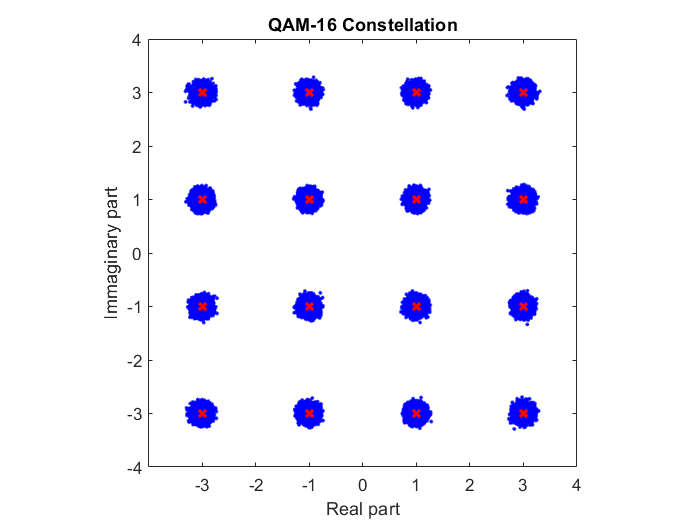
\includegraphics[width = .7\textwidth]{lab-6/imgs/SNR20.png}
\end{figure}
\vspace{-10px}

\FloatBarrier\noindent When the SNR reaches the value of 10, meaning that the signal is 10 times stronger than the noise the symbols start to move away from the red crosses. This is due to the fact that as the signal gets weaker the received symbols tend to differ from the source.

\begin{figure}[!h]
    \centering
    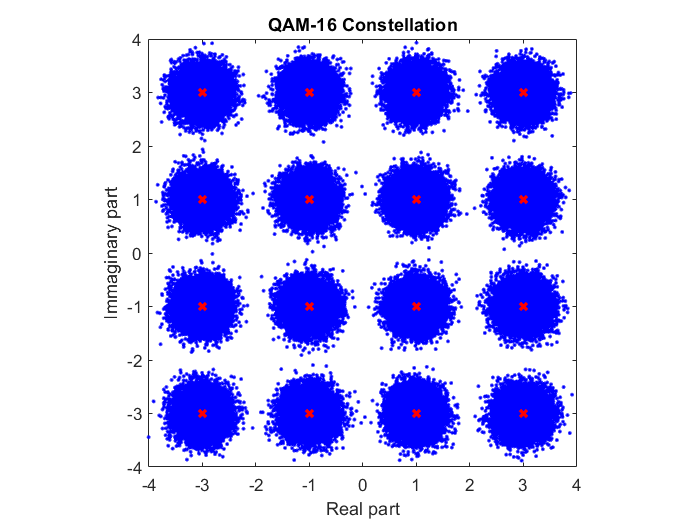
\includegraphics[width = .7\textwidth]{lab-6/imgs/SNR10.png}
\end{figure}
\vspace{-10px}

\FloatBarrier\noindent By decreasing the SNR value to 9, 8, 7 and 6 the blue constellation becomes larger and larger. When the SNR reaches the value of 7 and 6 some symbols start to overlap due to the excessive noisiness incurring in errors.

\begin{figure}[!h]
    \centering
    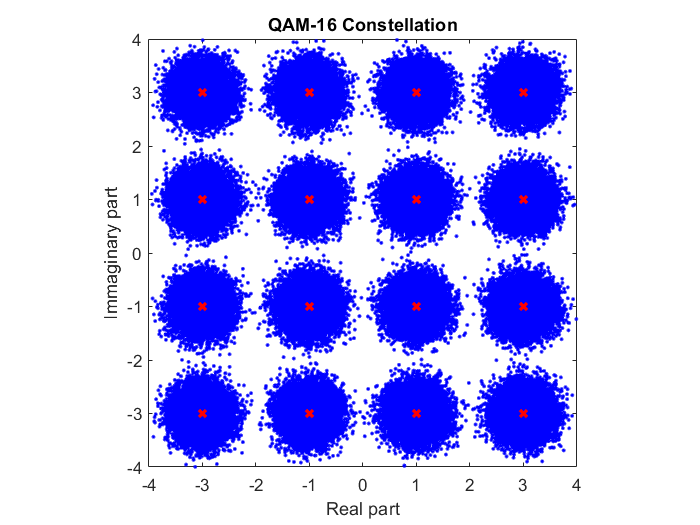
\includegraphics[width = .49\textwidth]{lab-6/imgs/SNR9.png}
    % \hspace*{5px}
    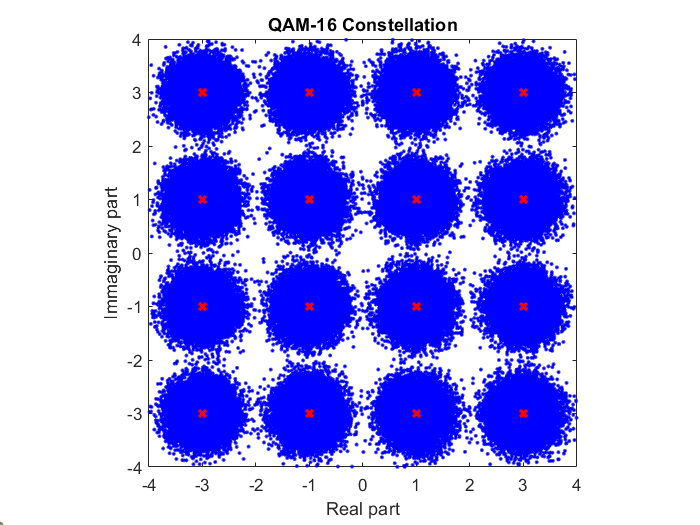
\includegraphics[width = .49\textwidth]{lab-6/imgs/SNR8.png}
    \\
    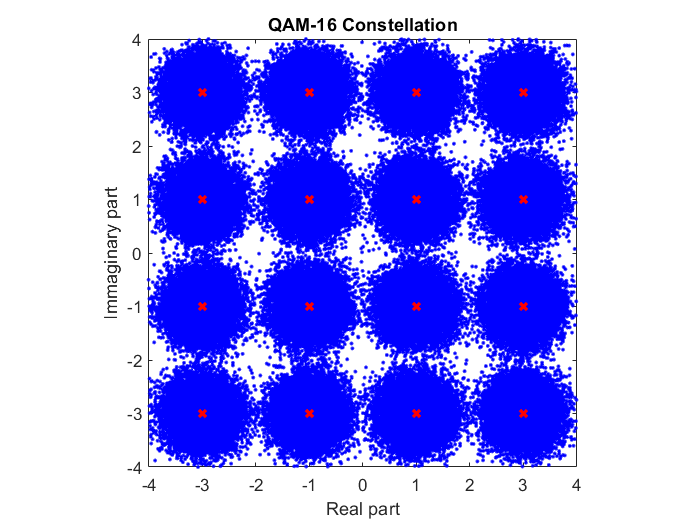
\includegraphics[width = .49\textwidth]{lab-6/imgs/SNR7.png}
    % \hspace*{5px}
    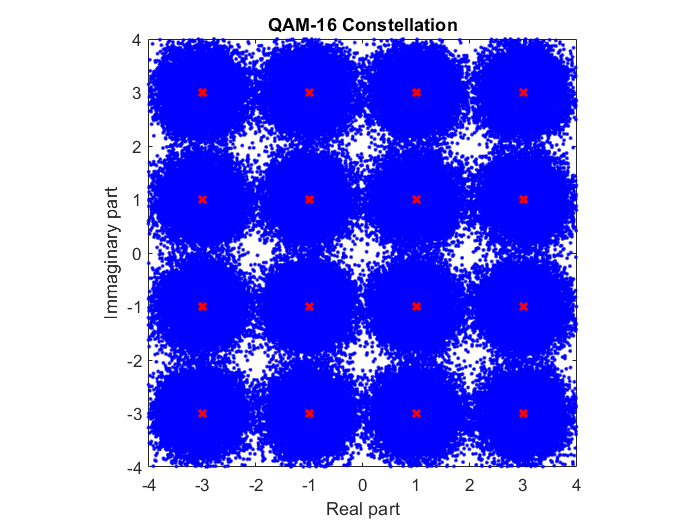
\includegraphics[width = .49\textwidth]{lab-6/imgs/SNR6.png}
\end{figure}
\vspace{-10px}

\FloatBarrier\noindent As the SNR reaches 5 the constellation begins to become a little less clear: the overlappings between the symbols start to increase and the disorder starts to be visible in the constellation. 
\begin{figure}[!h]
    \centering
    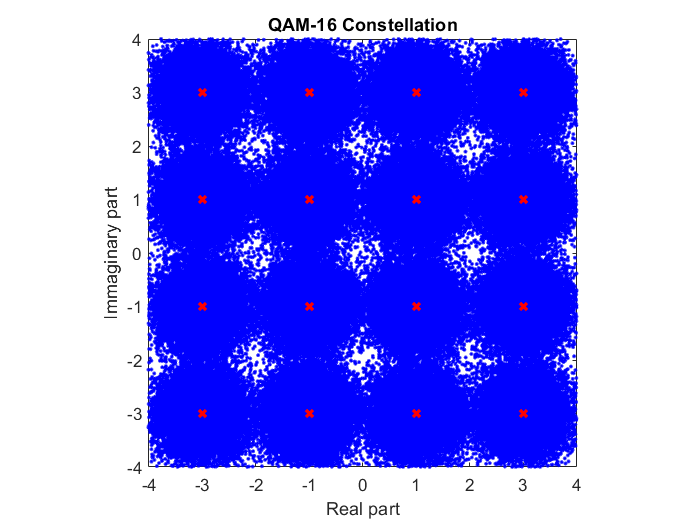
\includegraphics[width = .7\textwidth]{lab-6/imgs/SNR5.png}
\end{figure}
\vspace{-10px}


\FloatBarrier\noindent As the SNR approaches 0 the symbols are not recognisable anymore. This is because now the transmitted signal and the noise have the same energy. In such a way the symbols are all spread in the plane making it impossible to properly detect the correct symbol around the ideal one generating a cahotic constellation.

\begin{figure}[!h]
    \centering
    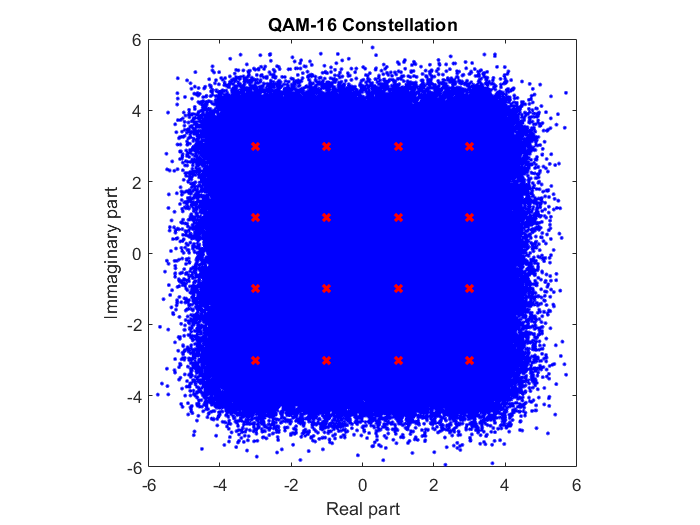
\includegraphics[width = .7\textwidth]{lab-6/imgs/SNR0.png}
\end{figure}
\vspace{-10px}

\FloatBarrier\subsection*{Task 3}
The third task's purpose is to numerically evaluate the BER (\textsl{Bit Error Rate}) and the number of errors. The first thing to do is to demodulate the received data using the script inside the file \texttt{demodData.m}.

Shortly, the script inside this file creates a matrix of 16 columns and $\frac{N}{4}$ rows that contain, per each column $i\in [1, 16]$, the distance between each symbol and the \textit{i-th} QAM-16 symbol. Secondly, every symbol is associated with a QAM-16 symbol based on its minimum distance value. Then the decimal value is converted into binary and formatted in a 4 by $\frac{N}{4}$ that will be used to compare with its original value.

\begin{lstlisting} 
% The script determines the binary sequence of each received QAM-16 symbol
% This is achieved by comparing absolute distance between received symbol and every possible QAM-16 constellation signal
% Note: The resulting binary data is stored in binDmd vector-row

% This approach requires replicating column of received symbols to create a matrix with dimensions N/4x16. "repmat()" function is used to do so.
symMtx = repmat(symNoi, 1, 16);

% Likewise, convert constellation vector into row and replicate it to match dimensions of symMtx matrix.
mapMtx = repmat(mapQAM16.', N/4, 1);     % Note ".'" transpose for complex values!

% Now calculate distances to each QAM-16 symbol for each row.
dstMtx = abs(symMtx - mapMtx);

% Finds minimum distance in each row and determine the column number of this minimum
% Finds minimums in rows (dimension 2)
[dstMin, symDmd] = min(dstMtx, [], 2);

% These minimum values are decimal representations (with added +1) of binary data. Performs BIN -> DEC conversion
binDmd = dec2bin(symDmd - 1, 4);         % Subtract -1 to set minimum symbol value to 0

% The output of the dec2bin function is a TEXT string. Performs logical comparison to obtain numerical values.
binDmd = (binDmd == '1')';

% Transposes matrix to dimensions 4xN/4 and unwraps matrix into single column
binDmd = binDmd(:)'; 
\end{lstlisting}

After adding this script, only two additional lines of code are needed to calculate and display the number of errors and the \textsl{Bit Error Rate}. To determine the first value, it is necessary to sum all the symbols that are different from the source for the BER is sufficient to divide the number of errors with the total number fo symbols \textit{N}.

\begin{lstlisting}
% Count number of errors by comparing vectors binDt and binDmd
numErr = sum(binDmd ~= binDt)
BERval = numErr/N          % Number of errors ratio to total number of bits N
\end{lstlisting}

\noindent The total number of errors and the BER value are summed up in the following table.

\begin{table*}[h!]
    \centering
    \renewcommand{\arraystretch}{1.5}
    \begin{tabular}{|c|c c|}
        \hline
        \textbf{SNR vlaue} & \textbf{\# errors} & \textbf{BER value} \\\hline\hline
        20 & 0 & 0 \\\hline
        10 & 3 & $3\cdot10^{-6}$ \\\hline
        9 & 29 & $2.9\cdot10^{-5}$ \\\hline
        8 & 150 & $1.5\cdot10^{-4}$ \\\hline
        7 & 579 & $5.79\cdot10^{-4}$ \\\hline
        6 & 1776 & $1.78\cdot10^{-3}$ \\\hline
        5 & 4430 & $4.43\cdot10^{-3}$ \\\hline
        0 & 59159 & $59.16\cdot10^{-3}$ \\\hline
    \end{tabular}
    \renewcommand{\arraystretch}{1}
\end{table*}

\noindent Expectably, as the SNR value decreases the number of errors and the \textsl{Bit Error Rate} increases. When the signal is 100 times stronger than the noise, no error occurs. When the SNR value starts to decrease the errors start to manifest: sure enough, the BER increases by two orders of magnitude and becomes to get bigger. When the SNR value is zero, meaning that the energy of the signal is the same as the energy of the noise there are nearly 60 thousand errors out of one million symbols: nearly 6\% of the transmitted data are wrongly detected.

\section*{Conclusions}
Through these simulations, we can conclude that the QAM-16 modulation, even though is very effective, is very sensible to the noise. This is a reasonable conclusion because the transmitted data are not binary anymore but there are 16 different values that the signal can transmit. This means that even if the noise is not so powerful there are more possibilities to wrongly detect a symbol because it is no more a binary choice. Consequently in this type of transmission having a very high SNR value is crucial to reach an optimal transmission otherwise, even if the signal is ten times stronger than the noise some errors may occur. 


\end{document}